% Study notes: step-by-step derivation of the detuned rotation-and-shear results.
% Build:  cd paper/notes && tectonic detuned_derivation.tex
% Numbers quoted here come from simulations/sim_detuned_shear.py (end results)
% and simulations/check_detuned_steps.py (individual steps).
\documentclass[11pt,letterpaper]{article}
\usepackage[margin=1in]{geometry}
\usepackage[T1]{fontenc}
\usepackage{lmodern}
\usepackage{amsmath,amssymb,graphicx,booktabs,microtype,enumitem}
\usepackage[font=small,labelfont=bf]{caption}
\setlength{\parindent}{0pt}
\setlength{\parskip}{6pt}
\newcommand{\nbar}{\bar{n}}
\newcommand{\ncrit}{n_{\rm crit}}
\newcommand{\Obar}{\bar{\Omega}}
\newcommand{\ket}[1]{|#1\rangle}
\newcommand{\bra}[1]{\langle#1|}
\newcommand{\braket}[2]{\langle#1|#2\rangle}
\newcommand{\numcheck}[1]{\par{\small\textit{Numerical check.} #1}\par}
\begin{document}

{\Large\bfseries Rotation and shear off resonance: step-by-step derivations}\\[4pt]
Study notes for the detuned Jaynes--Cummings results. Nguyen Khoi Nguyen (Alan), November 2026.

\rule{\textwidth}{0.4pt}

\section*{0. What is derived}
For a two-level atom, initially excited, interacting with a coherent field of $\nbar\gg1$ photons at
detuning $\Delta$:
\begin{enumerate}[nosep,leftmargin=2em,label=R\arabic*.]
\item the state is a sum of two branches, with weights $\cos^2(\vartheta/2)$ and $\sin^2(\vartheta/2)$ [eq.~\eqref{e17}];
\item the two field components rotate by $\mp\varphi$, with $\varphi = g^2t/\Obar$ [eq.~\eqref{e9}];
\item each is sheared by $s = \varphi\,\nbar/(\nbar+\ncrit)$ [eqs.~\eqref{e12}, \eqref{e15}];
\item the field purity between collapse and revival is $\tfrac12(1+\cos^2\vartheta)+\tfrac12\sin^4\vartheta\sin^2\varphi$ [eq.~\eqref{e20}];
\item the $k$th revival has amplitude $\sin^2\vartheta\,(1+\pi^2k^2\sin^4\vartheta)^{-1/4}$ [eq.~\eqref{e23}];
\item detecting the atom in $\ket{g}$ leaves a balanced cat with probability $\tfrac12\sin^2\vartheta$ and
      fidelity $(1+s^2/4)^{-1/2}$ [eqs.~\eqref{e25}, \eqref{e26}];
\item cavity loss multiplies that fidelity by $\tfrac12(1+e^{-\Gamma})$, with
      $\Gamma = (2\kappa\nbar^{3/2}/g\sin\vartheta)(\varphi-\tfrac12\sin2\varphi)$ [eqs.~\eqref{e29}, \eqref{e30}];
\item for a cat of fixed size, a larger resonant field is better than detuning [section~10].
\end{enumerate}
R1, R2 and R3 on resonance, the resonant limit of the fidelity in R6 (as the overlap of one component
with a coherent state), R5, and R7 on resonance are already in the literature (section~15). The rest was
not found there.

\textbf{Conventions.} $\hbar=1$. $\sigma_z\ket{e}=\ket{e}$, $\sigma_-=\ket{g}\bra{e}$. Phase space:
$a=(x+ip)/\sqrt2$, so the vacuum has variance $\tfrac12$ in $x$ and in $p$. The field starts in
$\ket{\alpha}$ with $\alpha=\sqrt{\nbar}$ real: $\ket{\alpha}=\sum_n c_n\ket{n}$,
$c_n=\sqrt{p_n}$, $p_n=e^{-\nbar}\nbar^n/n!$ (mean $\nbar$, variance $\nbar$).

\section*{1. Hamiltonian and exact solution}
In the frame rotating at the cavity frequency, with $\Delta=\omega_{\rm atom}-\omega_{\rm cavity}$,
\begin{equation}\label{e1}
H=\tfrac12\Delta\,\sigma_z+g\,(a^\dagger\sigma_-+a\,\sigma_+).
\end{equation}
$H$ couples $\ket{e,n}$ only to $\ket{g,n+1}$. In that pair of states it is the $2\times2$ matrix
\[
H_n=\begin{pmatrix}\Delta/2 & g\sqrt{n+1}\\ g\sqrt{n+1} & -\Delta/2\end{pmatrix}
=\frac{\Omega_n}{2}\bigl(\cos\vartheta_n\,\tau_z+\sin\vartheta_n\,\tau_x\bigr),
\]
where $\tau_{x,z}$ are Pauli matrices acting in the pair, and
\begin{equation}\label{e2}
\Omega_n=\sqrt{\Delta^2+4g^2(n+1)},\qquad \cos\vartheta_n=\frac{\Delta}{\Omega_n},\qquad
\sin\vartheta_n=\frac{2g\sqrt{n+1}}{\Omega_n}.
\end{equation}
Because $(\cos\vartheta\,\tau_z+\sin\vartheta\,\tau_x)^2=1$,
$e^{-iH_nt}=\cos(\Omega_nt/2)-i\sin(\Omega_nt/2)(\cos\vartheta_n\tau_z+\sin\vartheta_n\tau_x)$.
Acting on $\ket{e}\ket{\alpha}=\sum_nc_n\ket{e,n}$:
\begin{equation}\label{e3}
\ket{\psi(t)}=\sum_nc_n\Bigl\{\bigl[\cos\tfrac{\Omega_nt}{2}-i\cos\vartheta_n\sin\tfrac{\Omega_nt}{2}\bigr]\ket{e,n}
-i\sin\vartheta_n\sin\tfrac{\Omega_nt}{2}\,\ket{g,n+1}\Bigr\}.
\end{equation}
This is exact. For $\Delta=0$ it reduces to $\cos(gt\sqrt{n+1})$ and $-i\sin(gt\sqrt{n+1})$.

\section*{2. Two branches (still exact)}
Use $\cos\vartheta=\cos^2\tfrac\vartheta2-\sin^2\tfrac\vartheta2$ and
$\sin\vartheta=2\sin\tfrac\vartheta2\cos\tfrac\vartheta2$. With $u=\Omega_nt/2$,
\[
\cos u-i\cos\vartheta\sin u=\cos^2\tfrac\vartheta2\,e^{-iu}+\sin^2\tfrac\vartheta2\,e^{iu},\qquad
-i\sin\vartheta\sin u=\sin\tfrac\vartheta2\cos\tfrac\vartheta2\,(e^{-iu}-e^{iu}).
\]
Collecting the terms in $e^{-iu}$ and in $e^{iu}$ in eq.~\eqref{e3}:
\begin{equation}\label{e4}
\ket{\psi(t)}=\sum_nc_n\Bigl\{e^{-i\Omega_nt/2}\cos\tfrac{\vartheta_n}{2}\ket{+_n}
+e^{+i\Omega_nt/2}\sin\tfrac{\vartheta_n}{2}\ket{-_n}\Bigr\},
\end{equation}
\[
\ket{+_n}=\cos\tfrac{\vartheta_n}{2}\ket{e,n}+\sin\tfrac{\vartheta_n}{2}\ket{g,n+1},\qquad
\ket{-_n}=\sin\tfrac{\vartheta_n}{2}\ket{e,n}-\cos\tfrac{\vartheta_n}{2}\ket{g,n+1}.
\]
$\ket{\pm_n}$ are the dressed states, the eigenstates of $H_n$ with energies $\pm\Omega_n/2$.
Equation~\eqref{e4} says: $\ket{e,n}=\cos\tfrac{\vartheta_n}{2}\ket{+_n}+\sin\tfrac{\vartheta_n}{2}\ket{-_n}$,
and each dressed state only picks up a phase.

\section*{3. Large field: what may be replaced by its mean}
$p_n$ is concentrated within a few $\sqrt{\nbar}$ of $\nbar$. A quantity that changes little over
that range may be evaluated at $\nbar$: this applies to $\vartheta_n$ and to the difference between
$n$ and $n+1$ in amplitudes. It does \emph{not} apply to the phases $\Omega_nt/2$, because $t$ is
long enough for them to differ by many radians across the distribution. So expand the phase and
nothing else:
\begin{equation}\label{e5}
\Omega_n\simeq\Obar+\Omega'(n-\nbar)+\tfrac12\Omega''(n-\nbar)^2,\qquad
\Obar=\sqrt{\Delta^2+4g^2\nbar},\quad \Omega'=\frac{2g^2}{\Obar},\quad \Omega''=-\frac{4g^4}{\Obar^3}.
\end{equation}
Define the mixing angle at $\nbar$, the critical photon number, the rotation angle and the shear:
\begin{equation}\label{e6}
\sin\vartheta=\frac{2g\sqrt{\nbar}}{\Obar},\quad\cos\vartheta=\frac{\Delta}{\Obar},\qquad
\ncrit=\frac{\Delta^2}{4g^2}\ \Rightarrow\ \sin^2\vartheta=\frac{\nbar}{\nbar+\ncrit},
\end{equation}
\begin{equation}\label{e7}
\varphi\equiv\frac{g^2t}{\Obar},\qquad s\equiv\varphi\,\sin^2\vartheta .
\end{equation}
Since $g^4t/\Obar^3=\varphi\,g^2/\Obar^2=\varphi\sin^2\vartheta/4\nbar$, eq.~\eqref{e5} gives
\begin{equation}\label{e8}
\tfrac12\Omega_nt\simeq\tfrac12\Obar t+\varphi\,(n-\nbar)-\frac{s}{4\nbar}(n-\nbar)^2 .
\end{equation}
The three terms are: a common phase, a rotation, a shear. Define the two field states
$\ket{\Phi_\pm}\equiv\sum_nc_n\,e^{\pm i\Omega_nt/2}\ket{n}$; both are normalised.

\section*{4. First order: rotation}
Keep the first two terms of eq.~\eqref{e8}. Since $e^{i\varphi a^\dagger a}\ket{\alpha}=\ket{\alpha e^{i\varphi}}$,
\begin{equation}\label{e9}
\ket{\Phi_\pm}\simeq e^{\pm i(\Obar t/2-\varphi\nbar)}\,\ket{\alpha e^{\pm i\varphi}} .
\end{equation}
The two components are coherent states at angles $\pm\varphi$ on the circle of radius
$\sqrt{2\nbar}$ in the $(x,p)$ plane. Their separation in amplitude is
\begin{equation}\label{e10}
D=|\alpha e^{i\varphi}-\alpha e^{-i\varphi}|=2\sqrt{\nbar}\,|\sin\varphi|,\qquad
|\braket{\Phi_-}{\Phi_+}|\simeq e^{-D^2/2}=e^{-2\nbar\sin^2\varphi}\simeq e^{-g^2t^2\sin^2\vartheta/2}
\end{equation}
(the last form for small $\varphi$). This is the collapse: it takes $1/\sin\vartheta$ times longer
than on resonance.
\numcheck{At $gt\sin\vartheta=1$, $\nbar=100$, $\Delta=2g\sqrt{\nbar}$: exact 0.6080, formula 0.6065.}

\section*{5. Second order: shear}
Now the factor $\exp[\mp is(n-\nbar)^2/4\nbar]$. Rotate the frame so that the component lies on the
positive $x$ axis, and write $a=\sqrt{\nbar}+\delta a$. Then
\[
\hat n-\nbar=\sqrt{\nbar}\,(\delta a+\delta a^\dagger)+\delta a^\dagger\delta a\simeq\sqrt{2\nbar}\;\delta x,
\qquad \delta x=\frac{\delta a+\delta a^\dagger}{\sqrt2},
\]
where $\delta x$ is the \emph{radial} coordinate measured from the centre of the component. Hence
$(\hat n-\nbar)^2/4\nbar\simeq\delta x^2/2$, and the factor is the operator $e^{\mp is\,\delta x^2/2}$. A
coherent state has the wavefunction $\pi^{-1/4}e^{-\delta x^2/2}$, so
\begin{equation}\label{e11}
\psi_\pm(\delta x)=\pi^{-1/4}\exp\bigl[-\tfrac12(1\pm is)\,\delta x^2\bigr].
\end{equation}
Three things follow.

(i) $|\psi_\pm|^2$ is unchanged: the radial width stays at its vacuum value.

(ii) A phase $\theta(\delta x)$ on a wavefunction means a local momentum $d\theta/d\delta x$. Here
$\theta=\mp s\,\delta x^2/2$, so the tangential coordinate is shifted by $\mp s\,\delta x$: a
displacement along the circle proportional to the distance from it. This is a shear,
$(x,p)\to(x,\,p\mp sx)$, and it turns the covariance matrix $\tfrac12\,{\rm diag}(1,1)$ into
\begin{equation}\label{e12}
V_\pm=\frac12\begin{pmatrix}1&\mp s\\ \mp s&1+s^2\end{pmatrix}\qquad\text{in (radial, tangential) coordinates.}
\end{equation}
$\det V_\pm=\tfrac14$: the state is still pure and Gaussian, that is, a squeezed state. Its
eigenvalues are $\tfrac12e^{\mp2r}$ with
\begin{equation}\label{e13}
\cosh2r=1+\tfrac12s^2\quad\Longleftrightarrow\quad\sinh r=\tfrac12 s .
\end{equation}

(iii) The overlap with the coherent state at the same centre is one Gaussian integral:
\begin{equation}\label{e14}
\braket{\psi_0}{\psi_\pm}=\frac{1}{\sqrt\pi}\int e^{-(2\pm is)\delta x^2/2}\,d\delta x=\bigl(1\pm\tfrac{i}{2}s\bigr)^{-1/2},
\qquad|\braket{\psi_0}{\psi_\pm}|^2=\bigl(1+\tfrac14s^2\bigr)^{-1/2}.
\end{equation}

\textbf{Meaning.} The rotation rate of a component, $\Omega'/2=g^2/\Omega_n$, falls as $n$ grows. The
part of the component at larger radius therefore lags, and the part at smaller radius leads. With
eq.~\eqref{e6},
\begin{equation}\label{e15}
\boxed{\;s=\varphi\,\frac{\nbar}{\nbar+\ncrit}\;}
\end{equation}
On resonance the shear equals the rotation angle. Far off resonance it is smaller by $\nbar/\ncrit$.
\numcheck{Covariance of the exact $\ket{\Phi_+}$ in (radial, tangential) coordinates, $(V_{xx},V_{xp},V_{pp})$:
for $\nbar=1600$, $\Delta=0$, $\varphi=\pi/2$: $(0.501,-0.785,1.731)$ against $(0.500,-0.785,1.734)$;
for $\nbar=100$, $\Delta=2g\sqrt{\nbar}$, $\varphi=\pi/2$: $(0.502,-0.388,0.801)$ against $(0.500,-0.393,0.808)$.
The ratio $s/\varphi$ follows eq.~\eqref{e15} within 1\% for $\ncrit/\nbar$ from $10^{-2}$ to $10^{2}$ (figure~1d).}

\textbf{A lemma used repeatedly.} For a Gaussian variable $X$ with mean 0 and variance $\sigma^2$,
\begin{equation}\label{e16}
\bigl\langle e^{-iaX^2}\bigr\rangle=(1+2ia\sigma^2)^{-1/2}.
\end{equation}
Equation~\eqref{e14} is this with $\sigma^2=\tfrac12$ and $a=\pm s/2$.

\section*{6. The atom, and the purity of the field}
In eq.~\eqref{e4} replace $\vartheta_n$ by $\vartheta$. The $\ket{g,n+1}$ terms need one more step. Put
$m=n+1$: the term is $c_{m-1}e^{\pm i\Omega_{m-1}t/2}\ket{g,m}$. To leading order $c_{m-1}\simeq c_m$,
and $\Omega_{m-1}\simeq\Omega_m-\Omega'$, so
$e^{\pm i\Omega_{m-1}t/2}=e^{\pm i\Omega_mt/2}\,e^{\mp i\varphi}$ (because $\Omega't/2=\varphi$). One
photon more in the field costs a phase $\mp\varphi$. Therefore
\begin{equation}\label{e17}
\boxed{\;\ket{\psi(t)}\simeq\cos\tfrac\vartheta2\,\ket{\Phi_-}\ket{\chi_-}+\sin\tfrac\vartheta2\,\ket{\Phi_+}\ket{\chi_+}\;}
\end{equation}
\begin{equation}\label{e18}
\ket{\chi_-}=\cos\tfrac\vartheta2\ket{e}+e^{i\varphi}\sin\tfrac\vartheta2\ket{g},\qquad
\ket{\chi_+}=\sin\tfrac\vartheta2\ket{e}-e^{-i\varphi}\cos\tfrac\vartheta2\ket{g}.
\end{equation}
The branch weights are $\cos^2\tfrac\vartheta2=\tfrac12(1+\cos\vartheta)$ and
$\sin^2\tfrac\vartheta2=\tfrac12(1-\cos\vartheta)$. The two atomic states are not orthogonal:
\begin{equation}\label{e19}
\braket{\chi_-}{\chi_+}=\tfrac12\sin\vartheta\,(1-e^{-2i\varphi})=i\,e^{-i\varphi}\sin\vartheta\sin\varphi,
\qquad|\braket{\chi_-}{\chi_+}|=\sin\vartheta\,|\sin\varphi| .
\end{equation}
\numcheck{$1-|\langle\text{eq.~\eqref{e17}}|\text{exact}\rangle|^2$ lies between $0.9\times10^{-3}$ and
$4.3\times10^{-3}$ for $\nbar=100$ and between $2\times10^{-4}$ and $1.1\times10^{-3}$ for $\nbar=400$
(eight combinations of $\Delta$ and $\varphi$): an error of order $1/\nbar$. With the sign of
$\varphi$ in eq.~\eqref{e18} reversed the same quantity is between 0.2 and 1.}

\textbf{Purity.} After the collapse $\braket{\Phi_-}{\Phi_+}\simeq0$. Tracing out the atom from
eq.~\eqref{e17}, with $w_-=\cos^2\tfrac\vartheta2$ and $w_+=\sin^2\tfrac\vartheta2$,
${\rm Tr}\rho_{\rm field}^2=w_-^2+w_+^2+2w_-w_+|\braket{\chi_-}{\chi_+}|^2$. Using
$w_-^2+w_+^2=\tfrac12(1+\cos^2\vartheta)$ and $2w_-w_+=\tfrac12\sin^2\vartheta$,
\begin{equation}\label{e20}
{\rm Tr}\,\rho_{\rm field}^2=\tfrac12(1+\cos^2\vartheta)+\tfrac12\sin^4\vartheta\,\sin^2\varphi .
\end{equation}
On resonance this is $\tfrac12(1+\sin^2\varphi)$: it returns to 1 at $\varphi=\pi/2$, where
$\ket{\chi_+}=\ket{\chi_-}$ and the atom factors out. That is the disentanglement at half the
revival time. Off resonance the two atomic states never coincide, so the field is never pure
without a measurement.

\section*{7. Inversion and revivals}
From eq.~\eqref{e3}, $|c_{e}|^2-|c_{g}|^2$ summed over $n$ gives
\begin{equation}\label{e21}
\langle\sigma_z\rangle=\sum_np_n\bigl[\cos^2\vartheta_n+\sin^2\vartheta_n\cos\Omega_nt\bigr]
\simeq\cos^2\vartheta+\sin^2\vartheta\;{\rm Re}\,\braket{\Phi_-}{\Phi_+}.
\end{equation}
With eq.~\eqref{e8}, $\braket{\Phi_-}{\Phi_+}=\sum_np_ne^{i\Omega_nt}
=e^{i\Obar t}\sum_np_n\,e^{2i\varphi(n-\nbar)}\,e^{-is(n-\nbar)^2/2\nbar}$. The first factor in the sum
is the same for every integer $n$ when $2\varphi=2\pi k$:
\begin{equation}\label{e22}
t_k=\frac{k\pi\Obar}{g^2}\qquad(=2\pi k\sqrt{\nbar}/g\ \text{on resonance}).
\end{equation}
At $t_k$ the sum is the lemma \eqref{e16} with $\sigma^2=\nbar$ and $a=s/2\nbar$, that is $(1+is)^{-1/2}$
with $s=k\pi\sin^2\vartheta$. The oscillating part of the inversion therefore has amplitude
\begin{equation}\label{e23}
\sin^2\vartheta\,\bigl(1+\pi^2k^2\sin^4\vartheta\bigr)^{-1/4}.
\end{equation}
Geometrically: at a revival the two components sit on the same point but are sheared in opposite
senses, and the overlap of two Gaussian states is $|\braket{\Phi_-}{\Phi_+}|^2=\det(V_++V_-)^{-1/2}=(1+s^2)^{-1/2}$.
\numcheck{$\nbar=100$: $\Delta=0$: 0.5505 (formula 0.5507) for $k=1$, 0.3962 (0.3965) for $k=2$;
$\Delta=2g\sqrt{\nbar}$: 0.3663 (0.3664), 0.2752 (0.2754); $\Delta=4g\sqrt{\nbar}$: 0.1845 (0.1840), 0.1578 (0.1578).}

\section*{8. Detecting the atom: a heralded cat}
Project eq.~\eqref{e17} on $\ket{g}$, using eq.~\eqref{e18}:
\begin{equation}\label{e24}
\braket{g}{\psi}=\tfrac12\sin\vartheta\,\bigl(e^{i\varphi}\ket{\Phi_-}-e^{-i\varphi}\ket{\Phi_+}\bigr).
\end{equation}
After the collapse the two components are orthogonal, so the probability is
\begin{equation}\label{e25}
P_g=\tfrac14\sin^2\vartheta\times2=\tfrac12\sin^2\vartheta ,
\end{equation}
and the field is left in $(e^{i\varphi}\ket{\Phi_-}-e^{-i\varphi}\ket{\Phi_+})/\sqrt2$: a
\emph{balanced} superposition, whatever the detuning. Compare it with an ideal cat
$(\ket{\beta_-}+e^{i\theta}\ket{\beta_+})/\sqrt2$, $\beta_\pm=\alpha e^{\pm i\varphi}$. Each component
contributes the overlap \eqref{e14}, of modulus $(1+s^2/4)^{-1/4}$; choosing $\theta$ so that the two
contributions add in phase,
\begin{equation}\label{e26}
\boxed{\;F=\bigl(1+\tfrac14s^2\bigr)^{-1/2}\;}
\end{equation}
Finding the atom in $\ket{e}$ instead leaves $\cos^2\tfrac\vartheta2\ket{\Phi_-}+\sin^2\tfrac\vartheta2\ket{\Phi_+}$,
which is balanced only on resonance.

\textbf{No detection.} On resonance at $\varphi=\pi/2$ the atom factors out by itself and the field is
the same balanced superposition with $s=\pi/2$:
\begin{equation}\label{e27}
F=\bigl(1+\pi^2/16\bigr)^{-1/2}=0.786\quad\text{for }\nbar\to\infty,\text{ whatever the size of the cat}.
\end{equation}

\textbf{Two remarks.} The relative phase of the two components contains $\Obar t$, so it advances
at a rate of the order of the Rabi frequency: the timing of the detection fixes which cat is made.
This has not been quantified. And the sequence assumed here is an excited atom with the coupling
switched on suddenly; experiments near resonance often use adiabatic entry and Ramsey pulses,
for which the weights differ.
\numcheck{$\nbar=100$, exact / formula. Columns: purity \eqref{e20}, $P_g$ \eqref{e25}, $F$ \eqref{e26}.}
\begin{center}\small
\begin{tabular}{@{}cccccc@{}}
\toprule
$\Delta/2g\sqrt{\nbar}$ & $\varphi$ & $\sin^2\vartheta$ & purity & $P_g$ & $F$\\
\midrule
0 & $\pi/4$ & 1 & 0.7485 / 0.7500 & 0.5000 / 0.5000 & 0.9312 / 0.9308\\
0 & $\pi/2$ & 1 & 0.9957 / 1.0000 & 0.5000 / 0.5000 & 0.7881 / 0.7864\\
0.5 & $\pi/4$ & 0.8 & 0.7580 / 0.7600 & 0.4002 / 0.4000 & 0.9546 / 0.9540\\
0.5 & $\pi/2$ & 0.8 & 0.9171 / 0.9200 & 0.4002 / 0.4000 & 0.8484 / 0.8467\\
1 & $\pi/4$ & 0.5 & 0.8105 / 0.8125 & 0.2506 / 0.2500 & 0.9815 / 0.9813\\
1 & $\pi/2$ & 0.5 & 0.8732 / 0.8750 & 0.2506 / 0.2500 & 0.9316 / 0.9308\\
2 & $\pi/4$ & 0.2 & 0.9087 / 0.9100 & 0.1006 / 0.1000 & 0.9969 / 0.9969\\
2 & $\pi/2$ & 0.2 & 0.9188 / 0.9200 & 0.1006 / 0.1000 & 0.9878 / 0.9879\\
\bottomrule
\end{tabular}
\end{center}
The exact $F$ is the largest fidelity with any superposition $a_1\ket{\beta_1}+a_2\ket{\beta_2}$ of two
coherent states. Equation~\eqref{e26} is the overlap with coherent states at the centres of the
components; at finite $\nbar$ the best pair sits slightly off the centres, so the exact value is
usually slightly above the formula, most visibly at large $\varphi$: on resonance at $\varphi=\pi/2$ it is 0.802, 0.793
and 0.788 for $\nbar=10$, 25 and 100, approaching 0.786 from above as $0.16/\nbar$.

\section*{9. Cavity loss}
The master equation is $\dot\rho=-i[H,\rho]+\kappa\bigl(a\rho a^\dagger-\tfrac12\{a^\dagger a,\rho\}\bigr)$.

\textbf{Step 1: two coherent states.} Apply the loss term to $\rho_{12}=\ket{\beta_1}\bra{\beta_2}$ and
take the matrix element $\bra{\beta_1}\cdot\ket{\beta_2}$. Since $a\ket{\beta}=\beta\ket{\beta}$,
\[
\frac{d}{dt}\bra{\beta_1}\rho_{12}\ket{\beta_2}=\kappa\bigl(\beta_1\beta_2^*-\tfrac12|\beta_1|^2-\tfrac12|\beta_2|^2\bigr)
\bra{\beta_1}\rho_{12}\ket{\beta_2},
\]
and the real part of the bracket is $-\tfrac12|\beta_1-\beta_2|^2$. The coherence between two
coherent states decays at the rate
\begin{equation}\label{e28}
\tfrac12\kappa\,|\beta_1-\beta_2|^2 ,
\end{equation}
while each coherent state alone only shrinks, $\beta\to\beta e^{-\kappa t/2}$. (The exact result is
that the coherence is multiplied by $|\braket{\beta_2}{\beta_1}|^{\,1-e^{-\kappa t}}$; eq.~\eqref{e28} is its
short-time form.)

\textbf{Step 2: moving components.} Here $|\beta_+-\beta_-|^2=D^2=4\nbar\sin^2\varphi$ grows with time,
so the rate is $2\kappa\nbar\sin^2\varphi$. Integrate it, using $dt=(\Obar/g^2)\,d\varphi$:
\begin{equation}\label{e29}
\boxed{\;\Gamma=\int_0^t2\kappa\nbar\sin^2\varphi\,dt'=\frac{\kappa\nbar\Obar}{g^2}\bigl(\varphi-\tfrac12\sin2\varphi\bigr)
=\frac{2\kappa\nbar^{3/2}}{g\sin\vartheta}\bigl(\varphi-\tfrac12\sin2\varphi\bigr)\;}
\end{equation}
This assumes $\kappa t\ll1$ (the amplitude has not yet decayed) and treats the components as
coherent states when computing the rate. The loss acts on the field while the atom is still
entangled with it; the same factor $e^{-\Gamma}$ multiplies the coherence between the two branches
of eq.~\eqref{e17}.

\textbf{Step 3: the heralded state.} After detection of $\ket{g}$ the field is
$\tfrac12\bigl[\ket{\Phi_-}\bra{\Phi_-}+\ket{\Phi_+}\bra{\Phi_+}-e^{-\Gamma}\bigl(e^{2i\varphi}\ket{\Phi_-}\bra{\Phi_+}+{\rm h.c.}\bigr)\bigr]$, so
\begin{equation}\label{e30}
F=\bigl(1+\tfrac14s^2\bigr)^{-1/2}\;\tfrac12\bigl(1+e^{-\Gamma}\bigr),
\end{equation}
\begin{equation}\label{e31}
{\rm Tr}\,\rho_g^2=\tfrac12\bigl(1+e^{-2\Gamma}\bigr).
\end{equation}
On resonance at $\varphi=\pi/2$,
\begin{equation}\label{e32}
\Gamma=\pi\kappa\nbar^{3/2}/g ,
\end{equation}
which is the fringe-visibility formula of the manuscript.
\numcheck{Master equation / eq.~\eqref{e30}, cat size $D=6.32$, $\Delta=0$:}
\begin{center}\small
\begin{tabular}{@{}ccccc@{}}
\toprule
$\nbar$ & $\varphi$ & $\kappa/g=0.005$ & $\kappa/g=0.01$ & $\kappa/g=0.02$\\
\midrule
10 & 1.571 & 0.644 / 0.633 & 0.548 / 0.539 & 0.454 / 0.447\\
25 & 0.685 & 0.846 / 0.844 & 0.768 / 0.764 & 0.660 / 0.652\\
100 & 0.322 & 0.892 / 0.891 & 0.817 / 0.813 & 0.709 / 0.700\\
\bottomrule
\end{tabular}
\end{center}

\section*{10. A cat of fixed size: larger field or detuning?}
Fix $D=2\sqrt{\nbar}\sin\varphi$.

\textbf{On resonance}, any $\nbar\ge D^2/4$ will do, with $\varphi=\arcsin(D/2\sqrt{\nbar})$ and $s=\varphi$.
\begin{center}\small
\begin{tabular}{@{}lccc@{}}
\toprule
 & $F$ without loss & $\Gamma$ & $gt$\\
\midrule
smallest field, $\nbar=D^2/4$, $\varphi=\pi/2$ & 0.786 & $\pi\kappa D^3/8g$ & $\pi D/2$\\
large field, $\varphi\simeq D/2\sqrt{\nbar}\ll1$ & $1-D^2/32\nbar$ & $\kappa D^3/6g$ & $D$\\
\bottomrule
\end{tabular}
\end{center}
The second row uses $(1+\varphi^2/4)^{-1/2}\simeq1-\varphi^2/8$ and
$\varphi-\tfrac12\sin2\varphi\simeq\tfrac23\varphi^3$ in eq.~\eqref{e29}. The larger field is better on all
three counts; the exponent falls by the factor $3\pi/4=2.36$.

\textbf{Detuning at fixed $\nbar$ and $D$} (so $\varphi$ is fixed). Write $u=\sin\vartheta$ and let
$\Gamma_0$ be the resonant exponent. Then $s=\varphi u^2$ and $\Gamma=\Gamma_0/u$:
\[
F(u)=\bigl(1+\tfrac14\varphi^2u^4\bigr)^{-1/2}\,\tfrac12\bigl(1+e^{-\Gamma_0/u}\bigr),\qquad
\frac{d\ln F}{du}\Big|_{u=1}=-\frac{2\varphi^2}{4+\varphi^2}+\frac{\Gamma_0}{e^{\Gamma_0}+1}.
\]
Detuning means lowering $u$ from 1, so it raises $F$ only if this derivative is negative:
\begin{equation}\label{e33}
\frac{\Gamma_0}{e^{\Gamma_0}+1}<\frac{2\varphi^2}{4+\varphi^2}.
\end{equation}
For small $\varphi$ and $\Gamma_0$ this is $\Gamma_0<\varphi^2$; with $\Gamma_0\simeq\kappa D^3/6g$ and
$\varphi\simeq D/2\sqrt{\nbar}$,
\begin{equation}\label{e34}
\kappa D\nbar/g<\tfrac32 .
\end{equation}
Detuning also lowers the success probability to $\tfrac12u^2$. There is no universal optimal detuning.
\numcheck{$\nbar=25$, $D=6.32$: eq.~\eqref{e33} gives the threshold $\kappa/g=0.0121$ (eq.~\eqref{e34}: 0.0095). Master
equation / eq.~\eqref{e30} at $\Delta/2g\sqrt{\nbar}=0,\,1,\,2$: for $\kappa/g=0.002$: 0.904/0.902, 0.923/0.922,
0.899/0.900; for $\kappa/g=0.01$: 0.768/0.764, 0.749/0.740, 0.682/0.667.}

\section*{11. Three limits}
\textbf{(a) Resonance.} $\sin\vartheta=1$, $\Obar=2g\sqrt{\nbar}$, $s=\varphi=gt/2\sqrt{\nbar}$: the results
of the manuscript.

\textbf{(b) Dispersive regime,} $\Delta\gg2g\sqrt{\nbar}$. $\Obar\simeq\Delta$ and
$\varphi\simeq g^2t/\Delta$: the usual dispersive shift $g^2/\Delta$ of the cavity frequency. The
second-order phase in eq.~\eqref{e8} is $\mp(g^4t/\Delta^3)(n-\nbar)^2$: a Kerr term $\pm(g^4/\Delta^3)(a^\dagger a)^2$
in the Hamiltonian, and
\begin{equation}\label{e35}
s\simeq\varphi\,\nbar/\ncrit=4g^4\nbar t/\Delta^3 .
\end{equation}

\textbf{(c) Strong field at fixed $gt$.} Write $a=\sqrt{\nbar}+\delta a$ on resonance:
$H=g\sqrt{\nbar}\,\sigma_x+g(\delta a^\dagger\sigma_-+\delta a\,\sigma_+)$. With
$\sigma_\mp=\tfrac12(\sigma_x\mp i\sigma_y)$, the $\sigma_y$ parts rotate at $2g\sqrt{\nbar}$ under the
first term and average out, leaving
\begin{equation}\label{e36}
H_{\rm eff}=g\sqrt{\nbar}\,\sigma_x+\tfrac12g\,\sigma_x(\delta a+\delta a^\dagger).
\end{equation}
The field is displaced by $\mp igt/2$ according to $\sigma_x=\pm1$: a conditional displacement
with $D=gt$ and $\Gamma=\int\tfrac12\kappa(gt')^2dt'=\kappa D^3/6g$, the large-field row of section~10.
The shear is the first correction to this picture.

\section*{12. Where the approximations fail}
\begin{itemize}[nosep,leftmargin=1.5em]
\item \textbf{Finite $\nbar$.} Errors are of relative order $1/\nbar$ (section~6 check). At $\nbar=10$ on
      resonance the best two-coherent-state fidelity is 0.802 against the limit 0.786; at $\nbar=10$,
      $\Delta=2g\sqrt{\nbar}$ it is 0.936 against 0.931.
\item \textbf{Cubic term.} $\Omega'''=24g^6/\Obar^5$ adds a phase of order
      $\varphi\sin^4\vartheta/8\sqrt{\nbar}$ across the distribution. At $\varphi=\pi/2$ on resonance
      this is 0.06 for $\nbar=10$ and 0.02 for $\nbar=100$. It bends the components into crescents and
      ends the Gaussian picture after a number of revivals of order $\sqrt{\nbar}$.
\item \textbf{Before the collapse.} Equations \eqref{e20}, \eqref{e25}, \eqref{e26} need $e^{-2\nbar\sin^2\varphi}\ll1$.
\item \textbf{Loss.} Equation~\eqref{e30} is within about 1\% of the master equation for $\Gamma<1$ and
      $\kappa t\ll1$, and worsens beyond.
\item \textbf{Model.} Two-level atom and rotating-wave approximation. The formulas do not apply to a
      transmon in the dispersive regime, where higher levels change the Kerr term.
\item \textbf{Not included.} Atomic decay and dephasing, thermal photons, timing jitter.
\end{itemize}

\section*{13. Self-test}
Work these without notes.
\begin{enumerate}[nosep,leftmargin=1.5em]
\item Starting from $H_n$, derive eq.~\eqref{e3}. Check the limit $\Delta=0$.
\item Show that $\ket{e,n}=\cos\tfrac{\vartheta_n}{2}\ket{+_n}+\sin\tfrac{\vartheta_n}{2}\ket{-_n}$ and obtain eq.~\eqref{e4}.
\item Compute $\Omega'$ and $\Omega''$ and show that the quadratic phase is $s(n-\nbar)^2/4\nbar$ with $s=\varphi\sin^2\vartheta$.
\item Explain why $\vartheta_n$ may be replaced by $\vartheta$ but $\Omega_nt$ may not be replaced by $\Obar t$.
\item From $\psi(\delta x)\propto e^{-(1+is)\delta x^2/2}$ obtain the covariance matrix \eqref{e12}, the squeezing \eqref{e13} and the overlap \eqref{e14}.
\item Where does the factor $e^{\mp i\varphi}$ in $\ket{\chi_\pm}$ come from? What goes wrong in eq.~\eqref{e19} without it?
\item Derive the purity \eqref{e20} and say why the atom disentangles only on resonance.
\item Derive $P_g=\tfrac12\sin^2\vartheta$ and $F=(1+s^2/4)^{-1/2}$. Why is the heralded cat balanced for any detuning?
\item Derive the decoherence rate \eqref{e28} from the master equation, then $\Gamma$ in eq.~\eqref{e29}.
\item For fixed $D$, obtain the two rows of the table in section~10 and the criterion \eqref{e34}.
\item Recover the Kerr coefficient $g^4/\Delta^3$ and the conditional displacement \eqref{e36}.
\item Which of R1--R8 are already published, and where?
\end{enumerate}

\section*{14. Reproducing the numbers}
\begin{itemize}[nosep,leftmargin=1.5em]
\item \texttt{simulations/check\_detuned\_steps.py}\\ prints the step checks of sections 4--6 and 12 (a few seconds).
\item \texttt{simulations/sim\_detuned\_shear.py}\\ prints the tables of sections 7--10 and draws figure~1 (about a minute).
\end{itemize}

\section*{15. Where each piece already appears}
\begin{itemize}[nosep,leftmargin=1.5em]
\item Two branches and the atomic states on resonance: Gea-Banacloche, \emph{Phys.\ Rev.\ Lett.}\ \textbf{65}, 3385 (1990); \emph{Phys.\ Rev.}\ A \textbf{44}, 5913 (1991). With detuning: \emph{Opt.\ Commun.}\ \textbf{88}, 531 (1992), not yet read in full.
\item The second order on resonance (the quadratic phase; the squeezing of each component, equivalent to the covariance matrix and squeezing derived in section~5; its overlap with a coherent state, $(1+s^2/4)^{-1/2}$; the value 0.55 at the first revival): Gea-Banacloche, \emph{Phys.\ Rev.}\ A \textbf{44}, 5913 (1991), appendix~B, eqs.~(B4), (B11)--(B13), (B16)--(B18). The quadratic phase is also eq.~(2) of Auff\`eves \emph{et al.}, \emph{Phys.\ Rev.\ Lett.}\ \textbf{91}, 230405 (2003).
\item Revival envelope with detuning, eq.~\eqref{e23}: Feranchuk and Leonov, \emph{Phys.\ Lett.}\ A \textbf{373}, 517 (2009).
\item Loss exponent on resonance, eq.~\eqref{e29} with $\sin\vartheta=1$: Meunier \emph{et al.}, \emph{Phys.\ Rev.}\ A \textbf{74}, 033802 (2006), eq.~(45).
\item Decoherence rate \eqref{e28}: Walls and Milburn, \emph{Phys.\ Rev.}\ A \textbf{31}, 2403 (1985).
\item Kerr term \eqref{e35}: Boissonneault, Gambetta and Blais, \emph{Phys.\ Rev.}\ A \textbf{79}, 013819 (2009).
\item Conditional displacement \eqref{e36} with an external drive: Solano, Agarwal and Walther, \emph{Phys.\ Rev.\ Lett.}\ \textbf{90}, 027903 (2003).
\item Numerical value 0.787 for eq.~\eqref{e27}: Munhoz and Vidiella-Barranco, \emph{J.\ Mod.\ Opt.}\ \textbf{52}, 1557 (2005).
\end{itemize}

\begin{center}
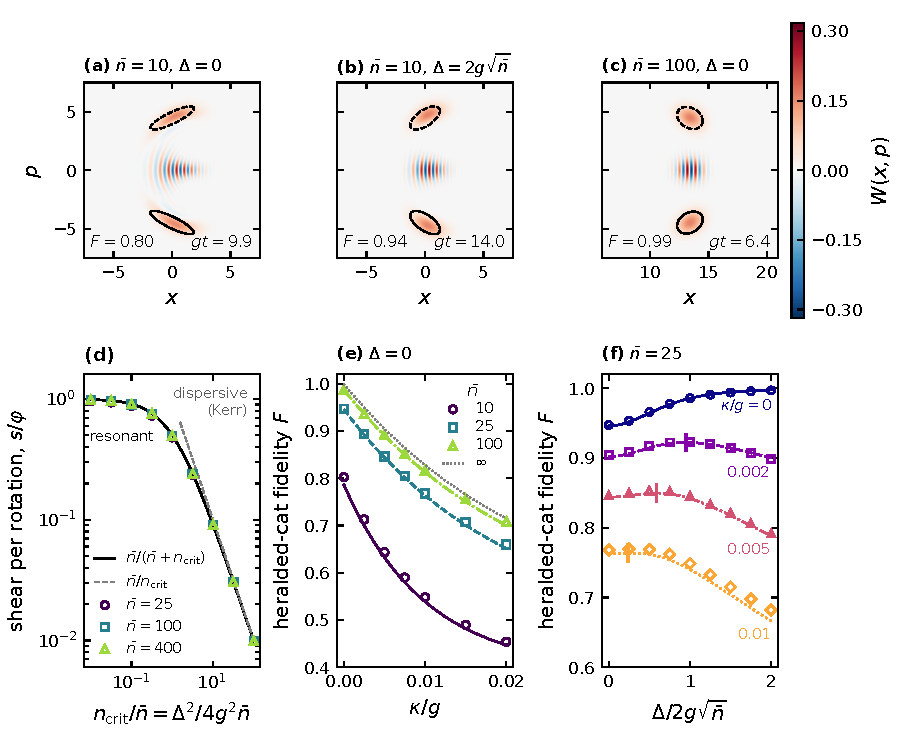
\includegraphics[width=0.92\textwidth]{../figures/fig_detuned_shear.pdf}
\end{center}
\vspace{-8pt}
\captionof{figure}{(a)--(c) A cat of the same size made three ways, atom detected in $\ket{g}$:
at half revival; with detuning; with a ten times larger field. Black curves: the ellipses of
eq.~\eqref{e12}. (d) Shear per unit rotation from the exact state (symbols) and eq.~\eqref{e15} (line).
(e) Fidelity against cavity loss at fixed cat size on resonance. (f) Fidelity against detuning at
fixed field and cat size; ticks mark the best detuning. In (e) and (f) symbols are master-equation
results and lines are eq.~\eqref{e30}.}

\end{document}
